%Stand: 31.08.2017

\documentclass[ngerman]{report}

\usepackage{BiVa}
\usepackage{mathmacros}
\usepackage{figures/tikz_pictures}
\usetikzlibrary{matrix}
\usepackage{caption}
\usepackage{listings}
\usepackage{stmaryrd}
\usepackage{pgfplots}
\usepackage{varwidth}
\usepackage[utf8]{inputenc}




\begin{document}

%%% tables and lists
\listoftodos
%\tableofcontents
%\listoftheorems

\chapter{1.Overview}

\begin{itemize}
	\item \enquote{image society} (webpages: 1995 text-based, 2005 image based, 
		2015 video based \dots)
		\begin{itemize}[-]
			\item data transfer rates $\uparrow$, compression rates $\uparrow$ 
			\item [critical shift: reading $\to$ watching]
		\end{itemize}
	\item \enquote{Photoshop}-ing \hfill (remove wrinkles, bumps, \dots)
	\item Images in medicine (\enquote{medical image proscessing}), x-ray, CT,
		MRI, ultrasound, \dots (\enquote{modalities}).\\
		different questions:
			\begin{enumerate}[1.)]
			  \item%
				\todoLayout{align bottom}
				\begin{minipage}{0.5\linewidth}
					measurments $\df[?]$ image\\
				  expl: tomography 	\\
					$\df$ difficult mathematical problems
				\end{minipage}
						\begin{minipage}{0.5\linewidth}
							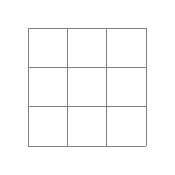
\begin{tikzpicture}[scale=0.5]
								\draw[help lines] (0,0) grid (3,3);
							\end{tikzpicture}
						\end{minipage}
				\item Image enhancements				
				\begin{itemize}

					\item denoising
						\begin{itemize}[]
							\item simple pixels/lines: 
							\todoWhat[so richtig?]
								\enquote{sandpaper} interpolation 
						  \item	global noise: smoothing		
						\end{itemize}

					\item grayscale
						\begin{itemize}[]
							\item histogramm balancing 
								(spreading)
						\end{itemize}

					\item distortion
						\begin{itemize}[]
							\item makes straight lines (in real world) straight 
								(in the images)
						\end{itemize}

					\item edge detection
						\begin{itemize}[]
						  \item contour enhancement 
						\end{itemize}

					\item segmentation
						\begin{itemize}[]
						  \item detect and separate parts of the image 
						\end{itemize}
					\item registration
						\begin{itemize}[]
						  \item \emph{sequence} of images of the same object 
								$\df$ \todomp{Wort?}, compare
								\begin{minipage}{0.3\linewidth}
									\todoSketch
								\end{minipage}
								$\nearrow$ object following in a movie
						\end{itemize}
				\end{itemize}
			\end{enumerate}
\end{itemize}

\textbf{\underline{Our Focus:}}
\begin{itemize}[-]
  \item mathematical models/methods/ideas 
	\item (algorthms)
	\item ((implementation))
\end{itemize}

\todoKom{skipped: Very fast intro: Matlab and images }	



\chapter{2.What is an image?}
\section{Discrete and continuous images}
There are (at least) two different points of view:
%%%%%%%%%%%%%%%%%%%%%%%%%%%
\def\leni{0.1\linewidth}
\def\lenii{0.45\linewidth}
\def\leniii{0.45\linewidth}
%%%%%%%%%%%%%%%%%%%%%%%%%%%

\begin{minipage}{\leni}
~	
\end{minipage}
\begin{minipage}{\lenii}
	$\bullet$ discrete/digital

	\begin{tikz}
		\draw[help lines] (0,0) grid (6,4);
	\end{tikz}
\end{minipage}
\begin{minipage}{\leniii}
	$\bullet$ continuous/analogue

	\begin{tikz}
		\draw[help lines] (0,0) grid (6,4);
	\end{tikz}
\end{minipage}

\begin{tabular}{p{\leni} p{\lenii} p{\leniii}}
	\textbf{object:} & matrix 															  & function \\
	\textbf{tools:}  & linear algebra (SVD, \dots) 					  & analysis (differentrage, integrate, 
		\dots) \\
	\textbf{pros:}   & (finite storage) storage, complexity   & freedom, tools,
		\todomp{motions?P.4} \par(e.g. edge discontinuity)\\
	\textbf{cons:}   & limitations: zooming, rotations, \dots & storage (infinite amout of data)\\
\end{tabular}

~\par
arguably, one has:

	\begin{itemize}
	  \item real life $\df$ continuous \enquote{images} (objects) 
		\item digital camers $\df$ discrete images
	\end{itemize}	

In general we will say:
\begin{definition}[(mathematical) image]
	A (mathematical) \emph{image} is a function	
		$$ u: \Omega \to F,$$
	\begin{tabbing}
	where: \= $\Omega \subset \Z^d$ (discrete) or $\Omega\subset \R^d$ (continuous) 
						\dots \emph{domain}\\
				 \> $d = 2$ (typical case 2D), $d=3$ (\enquote{3D image}=body or 
				 		$\underbrace{\text{2D+time}}_{\text{movie}}$)\\
				 \> $d = 4$ (3D + time) \par
	\end{tabbing}
	
	\begin{tabbing}
		$F$ \dots \= \emph{range of colours}\\
							\> $F= \R$ or $[0,\infty]$ or $[0,1]$  or $\set{0,\dots 255}$, \dots
								grayscale (light intensity) \\
							\> $F\subset \R^3$ \dots RGB image (colored)\\
							\> $F = \set{0,1}$ \dots black/white \hspace{2em}
							\begin{minipage}[c]{0.4\linewidth}
								\tikzpictureFourThree[scale=0.5]
							\end{minipage}
							\begin{minipage}[c]{0.3\linewidth}
								3 Layers\\
								$\df$ colored images:w
							\end{minipage}
	\end{tabbing}

\end{definition}

\todoKom{Matlab stuff}

Large parts of the course: analytical approach (i.e. continuous domain $\Omega$)\\
Since we want to differentirate, \dots the image $u$.
\begin{itemize}[]
  \item[Still:] need to assume that also $F$ ist continuous 
		(not as $\set{0,1}$, $\set{0,1,\dots,255}$ or $\N$)\\
		since otherwise the only differentiable (actually, the only continuous)
		functions $u: \Omega \to F$ are \emph{constant} functions 
		$\aq$ single-colour images
	\item[Also:] We usually take $F$ one-dimensional $(F \subset \R)$. 
		Think of it as either
			\begin{itemize}[-]
			  \item gray scaled image, or
				\item treating R,G \& B layer separately
			\end{itemize}
\end{itemize}

\section{Switching between discrete and continuous images}

\textbf{\large continuous $\to$ discrete:}\\
\begin{itemize}
  \item divide the continuous image in small squared pieces (boxes) 
	(superimpose grid) 

		\begin{minipage}[b]{0.6\linewidth}
		\hspace{-1em}$\bullet\;\:$now: represent each box by \emph{one} 
			value
			\begin{enumerate}[- str{a}tegy 1:]
			  \item take function value $u(x_i)$ \\
					\hspace{4em} for $x_i =$ midpoint of box $B_i$ 
				\item use mean value
					$$ \frac{1}{|B_i|}\int_{B_i} u(x) dx$$
			\end{enumerate}
		\end{minipage}%
		\begin{minipage}[t]{0.4\linewidth}
			\raisebox{1em}{\tikzpictureFIVEONE}
		\end{minipage}
\end{itemize}
$\df $ discrete image
\begin{enumerate}[str{a}tegy 1:]
  \item simple (and quick) but problemativ 
		($u(x_i)$ might represent $u|_{B_i}$ badly; 
		for $u\in L^p$, single point evaluation not
		even defined)
	\item more komplex but also more \enquote{democratic} 
		(actually closer to the way how CCD Sensors in 
		digital camers work)
\end{enumerate}
often the image value of the box $B_i$ gets also digitized, i.e.
fitted (by scaling \& rounding) into range $\set{0,1,dots,255}$
~\\
\par
\textbf{\large discrete $\to$ continous }\\

This is of course more tricky \dots

\begin{tabbing}
$\bullet$ Question:  $\quad$\= \kill

$\bullet$ Again: \> each pixel of the discrete image 
	 corresponds to a \enquote{box} of the continuous image \\
	\> (that is still to be constructed) \\

$\bullet$ Usually: \> pixel value $\mapsto$ \= function value at
	the \emph{midpoint} of the box \\
$\bullet$ Question: \> How to get the other function values 
	(in the box)?
\end{tabbing}

\hspace{1em}
\begin{minipage}[t][2cm][t]{0.30\textwidth}
	\tikzpictureSIXONE	 
\end{minipage}%
\begin{minipage}[c][2cm][t]{0.55\textwidth}
	\begin{tabbing}
 		\underline{idea 1:} $\;$ \= just take the function value of the 
			nearest\\ 
			\> midpoint (\enquote{nearest neighbour interpolation}) 
	\end{tabbing}
\end{minipage}
\vspace{-2.5em}
\begin{center}
For each $x\in B_i: u(x) := u(x_j) \;$ 
where $\displaystyle |x-x_j| = \min_{k} |x-x_k|$
\end{center}
\vspace{-.5em}
%
\begin{minipage}{0.3\linewidth}
 \tikzpictureSIXTWO
\end{minipage}
%
\begin{minipage}{0.7\linewidth}
		$\df \quad$ $u(x) = u(x_i)$ for all $x\in B_i$\\
		$\df \quad$ each box is uni-color\\
		$\df \quad$ the continuous image is essentially still discrete
\end{minipage}
~\\
~\\
{\underline{idea 2}: (bi-) lineare interpolation}



\chapter{3.Histogramm and first applicatsion}

\chapter{4.Basic Morphological Operations}

\chapter{5.Entrauschen: Filter und Co}
%This, again, is just a translation of my lecture note
%TODO move the tikz graphics into the dedicated directory
	\section{Noise}
		\mim{Noise} = Unwanted disturbances in an image. Mostly becaue of 
		\begin{enumerate}[-]
			\item point wise
			\item random
			\item independent
		\end{enumerate}
				We consider \emph{noise} to be an additive disturbances (for multiplicative noise use $log$).

		\emph{Notation:}
		\begin{center}
			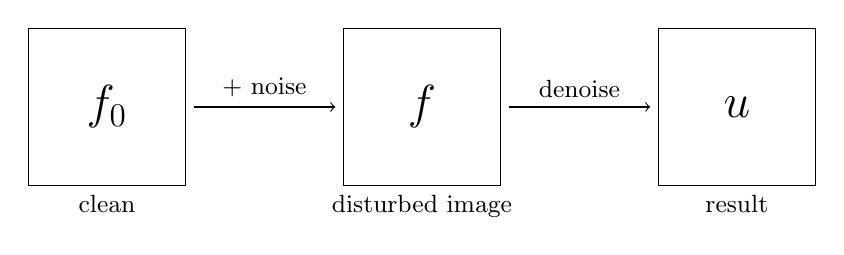
\begin{tikzpicture}
				\draw (0,0) rectangle (2,2);
				\draw (1,0) node[below] {\small clean};
				\draw (1,1) node[] {\LARGE $f_0$};
				\draw[->] (2.1,1) -- node[above] {\small $+$ noise} (3.9,1);
				\draw (4,0) rectangle (6,2);
				\draw (5,0) node[below] {\small disturbed image};
				\draw (5,1) node[] {\LARGE $f$};
				\draw[->] (6.1,1) -- node[above] {\small denoise} (7.9,1);
				\draw (8,0) rectangle (10,2);				
				\draw (9,0) node[below] {\small result};
				\draw (9,1) node[] {\LARGE $u$};
			\end{tikzpicture}
		\end{center}

		The quality of the denoised image $u$ compared to the original image $f_0$ is described by norms:
		\[
				\begin{aligned}
								\norm{f-f_0} & \dots \text{noise}\\
						\norm{u-f_0} & \dots \text{\mim{absolute error}}\\
						\frac{\norm{u-f_o}}{\norm{f-f_0}} & \dots \text{\mim{relative error} compared to the noise}\\
						\frac{\norm{u-f_o}}{\norm{f_0}} & \dots \text{relative error compared to the signal}
				\end{aligned}
				\]
		
		Typically the chosen norm is:
		\[\norm{f} = \norm{f}_2 = \sqrt{\int_{\Omega} \abs{f(x)}^2 dx}\]
		or in the discrete:
		\[\norm{f}_2=\sqrt{\sum_{x \in \Omega} \abs{f(x)}^2}\]

		Closely connected is the \mim{Signal to noise ratio} (SNR):
		\[log(\underbrace{\frac{\norm{f_0}_2}{\norm{u-f_0}_2}}_{\in \ [1,\infty)}) \in [0,+\infty), \text{ where $0$ is bad and $+\infty$ is good.}\]
	\section{smoothing filter}
		Idea: (to simplify in 1D)
		\begin{center}
			\begin{tikzpicture}
				\draw (0,0) node[left] {$f_0$:};
				\draw[thick] plot [smooth, tension = 0.7] coordinates {(0,0) (1.75,1.5) (3.5,0.5) (6,2) (9,0) (11,0.5)};
				\draw[->,thick] (-0.3,-0.5) -- node[left] {noise} (-0.3,-2);
				\draw (0,-2.5) node[left] {$f$:};				
				\draw[thick, name path = P2,shift = {(0,-2.5)}] plot [smooth, tension = 0.7] coordinates {(0,0) (1.75,1.5) (3.5,0.5) (6,2) (9,0) (11,0.5)};
				\draw[name path = P1, draw = none] (0,-1.1) -- (3,-1.1);
				\draw[name intersections={of = P1 and P2},red,thick]
				(intersection-1) edge[bend right] ++(0.3,0.5) ++(0.3,0.5) edge[bend right] (intersection-2);
				\draw[name path = P3,draw = none] (3,-2.3) -- (5,-1.2);
				\draw[name intersections={of = P3 and P2},red,thick]
				(intersection-1) edge[bend left] ++(0.3,-0.3) ++(0.3,-0.3) edge[bend left] (intersection-2);
				\draw[] (2,-0.9) -- ++(0.5,-0.1) node[right] {\small disturbances} (3.5,-2.1) -- ++(-0.5,0.9);
				\draw (0,-5) node[left] {$f$:};
				\draw[thick, name path = P4,shift = {(0,-5)}] plot [smooth, tension = 0.7] coordinates {(0,0) (1.75,1.5) (3.5,0.5) (6,2) (9,0) (11,0.5)};
				\draw[name path = P5, shift = {(0,-2.5)}, draw = none] (0,-1.1) -- (3,-1.1);
				\draw[name intersections={of = P4 and P5},red,thick]
				(intersection-1) edge[bend right] node[black,pos=0] {\small \textbullet} ++(0.3,0.5) ++(0.3,0.5) edge[bend right] node[black,pos=1] {\small \textbullet}  node[black,pos=0] {\small \textbullet} (intersection-2);
				\draw[name path = P6, shift = {(0,-2.5)}, draw = none] (3,-2.3) -- (5,-1.2);
				\draw[name intersections={of = P4 and P6},red,thick]
				(intersection-1) edge[bend left] node[black,pos=0] {\small \textbullet} ++(0.3,-0.3) ++(0.3,-0.3) edge[bend left] node[black,pos=1] {\small \textbullet}  node[black,pos=0] {\small \textbullet} (intersection-2);
				\draw[decorate,decoration={brace,amplitude=2pt,mirror}] (1.4,-3.7) -- (2.2,-3.7);
				\draw[thick] (1.8,-3.8) -- (1.8,-4.3) node[below] {\small \framebox{average}};
				\draw[->,thick,double] (1.6,-5) -- (0.4,-5);
				\draw[->,thick,double] (2,-5) -- (3.2,-5);
				\draw[->,thick] (1.8,-5.1) -- (1.8,-5.7);
				\draw (0,-7.5) node[left] {$u$:};
				\draw[->,thick] (-0.3,-5.5) -- node[left] {denoising} (-0.3,-7);
				\draw[thick, name path = P7,shift = {(0,-7.5)}] plot [smooth, tension = 0.7] coordinates {(0,0) (1.75,1.5) (3.5,0.5) (6,2) (9,0) (11,0.5)};
				\draw[name path = P8, shift = {(0,-5)}, draw = none] (0,-1.2) -- (3,-1.2);
				\draw[name intersections={of = P7 and P8},red,thick]
				plot [smooth,tension=0.7] coordinates {(intersection-1) ($(intersection-1) + (0.5,0.35)$) (intersection-2)};
				\draw[name path = P9, shift = {(0,-5)}, draw = none] (3,-2.25) -- (5,-1.15);
				\draw[name intersections={of = P7 and P9},red,thick]
				plot [smooth,tension=0.7] coordinates {(intersection-1) ($(intersection-1) + (0.45,0.05)$) (intersection-2)};
			\end{tikzpicture}
		\end{center}

		\begin{equation} \label{eq:5.1}
			u(k):=\alpha \cdot f(k-1) + \beta \cdot f(k) + \gamma \cdot f(k+1)
		\end{equation}
		where:
		\begin{equation} \label{eq:5.2}
			\alpha + \beta + \gamma = 1
		\end{equation}

		More precisely \eqref{eq:5.1} means:
		
		\begin{center}
			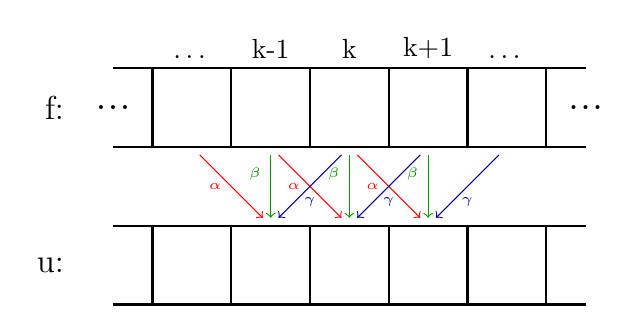
\begin{tikzpicture}
				\draw (0,-0.5) node[left] {\large f:};
				\draw[thick] (0.5,0) grid (6.5,-1);
				\draw (0.5,-0.5) node {\LARGE ...};
				\draw (6.5,-0.5) node {\LARGE ...};
				\draw (1.5,0) node[above] {\dots};
				\draw (2.5,0) node[above] {k-1};
				\draw (3.5,0) node[above] {k};
				\draw (4.5,0) node[above] {k+1};
				\draw (5.5,0) node[above] {\dots};

				\draw[->,red] (1.6,-1.1) -- node[left] {\tiny $\alpha$} (2.4,-1.9);
				\draw[->,red] (2.6,-1.1) -- node[left] {\tiny $\alpha$} (3.4,-1.9);
				\draw[->,red] (3.6,-1.1) -- node[left] {\tiny $\alpha$} (4.4,-1.9);
				\draw[->,black!40!green] (2.5,-1.1) -- node[left, pos = 0.3] {\tiny $\beta$} (2.5,-1.9);
				\draw[->,black!40!green] (3.5,-1.1) -- node[left, pos = 0.3] {\tiny $\beta$} (3.5,-1.9);
				\draw[->,black!40!green] (4.5,-1.1) -- node[left, pos = 0.3] {\tiny $\beta$} (4.5,-1.9);
				\draw[->,black!40!blue] (3.4,-1.1) -- node[right, pos = 0.75] {\tiny $\gamma$} (2.6,-1.9);
				\draw[->,black!40!blue] (4.4,-1.1) -- node[right, pos = 0.75] {\tiny $\gamma$} (3.6,-1.9);
				\draw[->,black!40!blue] (5.4,-1.1) -- node[right, pos = 0.75] {\tiny $\gamma$} (4.6,-1.9);

				\draw (0,-2.5) node[left] {\large u:};
				\draw[thick] (0.5,-2) grid (6.5,-3);
			\end{tikzpicture}
		\end{center}

		\begin{center}
			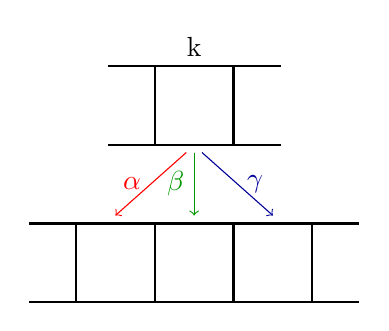
\begin{tikzpicture}
				\draw (0.5,0) node[above] {k};
				\draw[thick] (-0.6,0) grid (1.6,-1);
				\draw[->,red] (0.4,-1.1) -- node[left] {$\alpha$} (-0.5,-1.9);
				\draw[->,black!40!green] (0.5,-1.1) -- node[left] {$\beta$} (0.5,-1.9); 
				\draw[->,black!40!blue] (0.6,-1.1) -- node[right] {$\gamma$} (1.5,-1.9); 
				\draw[thick] (-1.6,-2) grid (2.6,-3);
			\end{tikzpicture}
		\end{center}

		With \eqref{eq:5.1} there is a mapping $f \mapsto u$, we write
		\[u = m \boxast f, \ \text{this is called \mim{Correlation}.}\]%TODO is it really correlation?
		where:
		\begin{equation}\label{eq:5.3}
			\framebox{$\displaystyle (m \boxast f)(k) = \sum_{i \in supp(m)} m(i) f(k+i)$}
		\end{equation}
		and:
		\begin{center}
			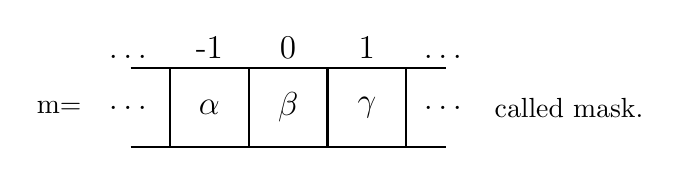
\begin{tikzpicture}
				\draw (0,0.5) node[left] {m=};
				\draw[thick] (0.5,0) grid (4.5,1);
				\draw (0.5,0.5) node {\large \dots};
				\draw (1.5,0.5) node {\large $\alpha$};
				\draw (2.5,0.5) node {\large $\beta$};
				\draw (3.5,0.5) node {\large $\gamma$};				
				\draw (4.5,0.5) node {\large \dots};
				\draw (0.5,1) node[above] {\large \dots};
				\draw (1.5,1) node[above] {\large -1};
				\draw (2.5,1) node[above] {\large 0};
				\draw (3.5,1) node[above] {\large 1};				
				\draw (4.5,1) node[above] {\large \dots};
				\draw (5,0.5) node[right] {called \mim{mask}.};
			\end{tikzpicture}
		\end{center}

		If you set $j:= k + i$ in \eqref{eq:5.1}, then $i=j-k$, which means:
		\begin{equation}\label{eq:5.4}
			\framebox{$\displaystyle (m \boxast f)(k) = \sum_{i \in supp(m)} m(j-k) f(j)$}
		\end{equation}

		To apply the mapping onto the boundary the image is reflected, in 1D:
		\begin{center}
			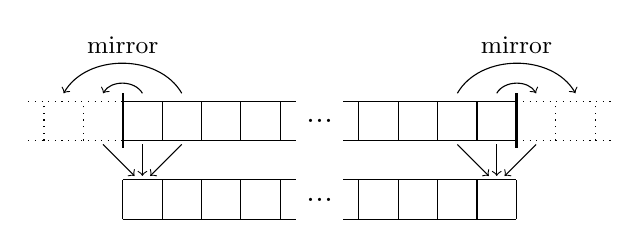
\begin{tikzpicture}
				\draw[step = 0.5] (0,0) grid (2.2,-0.5);
				\draw (2.5,-0.25) node {\large ...};
				\draw[step = 0.5] (2.8,0) grid (5,-0.5);
				\draw[thick] (0,0.1) -- (0,-0.6);
				\draw[thick] (5,0.1) -- (5,-0.6);
				\draw[step = 0.5, dotted] (0,0) grid (-1.2,-0.5);
				\draw[step = 0.5, dotted] (5,0) grid (6.2,-0.5);
				\draw[] (0.25,0.1) edge[bend right = 60, ->] (-0.25,0.1);
				\draw[] (0.75,0.1) edge[bend right = 60, ->] node[above] {\small mirror} (-0.75,0.1);
				\draw[] (4.75,0.1) edge[bend left = 60, ->] (5.25,0.1);
				\draw[] (4.25,0.1) edge[bend left = 60, ->] node[above] {\small mirror} (5.75,0.1);
				\draw[step = 0.5] (0,-1) grid (2.2,-1.5);
				\draw (2.5,-1.25) node {\large ...};
				\draw[step = 0.5] (2.8,-1) grid (5,-1.5);
				\draw[->] (0.25,-0.55) -- (0.25,-0.95);
				\draw[->] (-0.25,-0.55) -- (0.15,-0.95);
				\draw[->] (0.75,-0.55) -- (0.35,-0.95);
				\draw[->] (4.75,-0.55) -- (4.75,-0.95);
				\draw[->] (4.25,-0.55) -- (4.65,-0.95);
				\draw[->] (5.25,-0.55) -- (4.85,-0.95);
			\end{tikzpicture}
		\end{center}

		in 2D:

		\begin{center}
			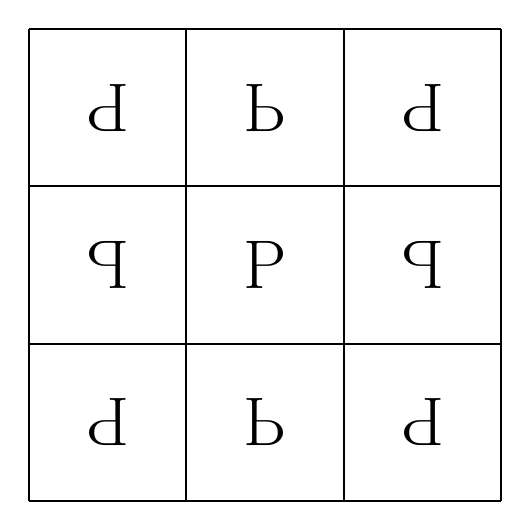
\begin{tikzpicture}
				\draw[step =2, thick] (0,0) grid (6,6);
				\draw (3,3) node {\Huge P};
				\draw (1,1) node[rotate = 180] {\Huge P};
				\draw (5,1) node[rotate = 180] {\Huge P};
				\draw (1,5) node[rotate = 180] {\Huge P};
				\draw (5,5) node[rotate = 180] {\Huge P};
				\draw (3,5) node[yscale=-1,xscale=1] {\Huge P};
				\draw (5,3) node[rotate = 180,yscale=-1,xscale=1] {\Huge P};
				\draw (1,3) node[rotate = 180,yscale=-1,xscale=1] {\Huge P};
				\draw (3,1) node[yscale=-1,xscale=1] {\Huge P};
			\end{tikzpicture}
		\end{center}

		Formula \eqref{eq:5.4} might remind one of the \mim{convolution}:
		\todoLayout
		\begin{equation}\label{eq:5.5}
			\framebox{$\displaystyle (g * f)(k) = \sum_{j \in \Z} g(\underbrace{k-j}_{\text{Difference to \eqref{eq:5.4}}}) \cdot f(j)$}
		\end{equation}

		If you set $g(i) := m(-i) =: \tilde m(i)$, which corresponds to 
		a reflection of the Mask, then
		\[m \boxast f = g * f = \tilde m * f\]
		\todoKom{Im Skript hier noch Beispiele und soetwas p. 32f}
		Properties of the convolution:
		\begin{enumerate}
			\item $(f * g) * h = f * (g* h)$, Associativity
			\item $f*g=g*f$, Commutativity
			\item $\tilde f * \tilde g = \widetilde{f * g}$, 
				Compatibility with reflection
		\end{enumerate}
		
		Properties of the correlation:
		\begin{enumerate}
			\item $f \boxast (g \boxast h) = \tilde f * ( \tilde g* h) 
				\overset{\framebox{\small 1}}{=} ( \tilde f * \tilde g) * h
				\overset{\framebox{\small 3}}{=} (\widetilde{f * g}) * h = 
				(f * g) \boxast h \neq (f \boxast g) \boxast h$, not associative!
			\item $f \boxast g = \tilde f * g \overset{
				\framebox{\small 2}}{=} g * \tilde f = 
					\tilde{\tilde g} * \tilde f \overset{\framebox{\small 3}}{=}
					\widetilde{(\tilde g * f)} = 
					\widetilde{g \boxast f} \neq g \boxast f$, not commutative!
			\item $\tilde f \boxast \tilde g = 
				\tilde{\tilde f} * \tilde g \overset{\framebox{\small 3}}{=}
				\widetilde{(\tilde f * g)} = \widetilde{f \boxast g}$, 
				Compatibility with reflection
		\end{enumerate}

		$\boxast$ und $*$ definiert man auf: 
			$\ell^1(\Z^d):=\set{f=(f_i)_{i \in \Z^d} : \underbrace{\sum_{
				i \in \Z^d}\abs{f_i}}_{:=\norm{f}_1} < \infty}$
		
			Man kann zeigen (Übung): $f,g \in \ell^1 \Rightarrow f * g \in \ell^1$ 
			und $\norm{f * g}_1 \leq \norm{f}_1 \cdot \norm{g}_1$.
			Wobei oft die Gleichheit gilt.
			
			Alles gilt auch in der Kontinuierlichen Version:
			\[L^1(\R^d) := \set{f:\R^d \to \R : 
				\underbrace{\int_{\R^d}\abs{f} dx}_{:=\norm{f}_1} < \infty} \]
			\[f,g \in L^1(\R^d): (g*f)(x)=\int_{\R^d}g(x-y)f(y) dy, \ y,x \in \R^d\]
		
			Beispiel für den kontinueirlichen Fall:
			\begin{center}
				\begin{tikzpicture}
					\draw[dotted] (0,1) node[left] {$\frac{1}{2a}$} -- (8,1);
					\draw (0,0) node[left] {$g:$} -- (2.5,0) -- (2.5,1) -- (5.5,1) -- (5.5,0) -- (8,0);
					\draw (2.5,0) node[below] {\small $-a$};
					\draw[dotted] (4,0) node[below] {\small $0$} -- (4,1.5);
					\draw (5.5,0) node[below] {\small $-a$};
				\end{tikzpicture}
			\end{center}
			Hierbei gilt $\displaystyle \int_{\R} g(x) dx = 1$
		
			\begin{center}
				\begin{tikzpicture}
					\draw[thick, name path = P2,shift = {(0,-2.5)}] node [left] {$f:$}plot [smooth, tension = 0.45] coordinates {(0,0) (1.2,1.5) (2.1,0.3) (3,2) (4.3,1) (5.3,1.6) (6.6,0.5) (7.5,1) (8,0)};
				\end{tikzpicture}
			\end{center}
		
			$g \boxast f = $ \mim{gleitendes Mittel}.\\
		
				\begin{tikzpicture}
					\draw[dotted] (0,1) node[left] {$\frac{1}{2a}$} -- (8,1);
					\draw (0,0) node[left] {$g \boxast g = \tilde g * g = g * g=$} -- (1,0) -- (4,1) -- (7,0) -- (8,0);
					\draw (1,0) node[below] {\small $-2a$};
					\draw[dotted] (4,0) node[below] {\small $0$} -- (4,1.5);
					\draw (7,0) node[below] {\small $-2a$};
				\end{tikzpicture}
		
			\todoLayout
			Weitere Eigenschaften der Faltung:\\
			Für alle $f,g \in L^1$ or $\ell ^1$
			\begin{equation*}
				\left.\begin{aligned}
					(g_1 + g_2) * f = (g_1 * f) + (g_2 * g)\\
					(\alpha g) * f = \alpha (g * f)
				\end{aligned}\right\}=\text{Linearität}
			\end{equation*}
			Somit ist:
			\[g \mapsto f * g\]
			ein linearer Operator.
		
			Formt $\ell^1$ bzw. $L^1$ eine Algebra mit neutralem Element $\delta$?
		
			$\ell^1$?:
			\begin{center}
				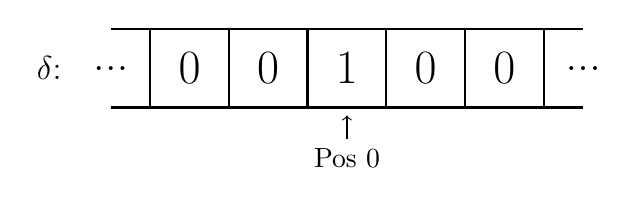
\begin{tikzpicture}
					\draw (0,-0.5) node[left] {\large $\delta$:};
					\draw[thick] (0.5,0) grid (6.5,-1);
					\draw (0.5,-0.5) node {\LARGE ...};
					\draw (6.5,-0.5) node {\LARGE ...};
					\draw (1.5,-0.5) node {\LARGE 0};
					\draw (2.5,-0.5) node {\LARGE 0};
					\draw (3.5,-0.5) node {\LARGE 1};
					\draw (4.5,-0.5) node {\LARGE 0};
					\draw (5.5,-0.5) node {\LARGE 0};
					\draw[->] (3.5,-1.4) node[below] {Pos $0$} -- (3.5,-1.1);
				\end{tikzpicture}
			\end{center}
			Ja!
		
			$L^1$?:
			Für ein solches Element muss gelten:\\
			$\forall f \in L^1 : d * f = f$\\
			$\forall x \in \R :\displaystyle \int_{\R^d} \underbrace{\delta(x-y)}_{=0 \forall x \neq y} f(y) dy = f(x)$
		
			Diese Funktion wird \mim{Dirac-Impuls} gennant ist aber kein Element von $L^1$.
		
			\underline{Nun zu Masken in 2D:}
		
			\begin{equation*}
				u = m \boxast f \text{ mit } m= \raisebox{-0.665cm}{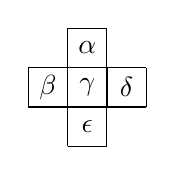
\begin{tikzpicture}
					\draw[step = 0.5] (0,0) grid (0.5,1.5);
					\draw[step = 0.5] (-0.5,1) grid (1,0.5);
					\draw (0.25,1.25) node {$\alpha$};
					\draw (0.25,0.75) node {$\gamma$};
					\draw (0.25,0.25) node {$\epsilon$};
					\draw (-0.25,0.75) node {$\beta$};
					\draw (0.75,0.75) node {$\delta$};
				\end{tikzpicture}}
			\end{equation*}
			wobei $\alpha + \beta +\gamma +\delta + \epsilon = 1$\\
			Kurzschreibweise: $u_{ij}:=u(x)$ wobei $x = \begin{pmatrix}i\\j\end{pmatrix} \in \Z^2$, analog für $f_{ij}$.
		
			\[\Rightarrow u_{ij} = \alpha f_{i-1,j} + \beta f_{i,j-i} + \gamma f_{ij} + \delta f_{i,j+1} + \epsilon f_{i+1,j}\]
		
			\begin{equation*}
				u = m \boxast f = \tilde m * f \text{ mit } \tilde m = \raisebox{-0.665cm}{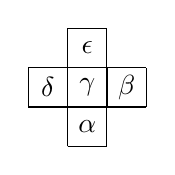
\begin{tikzpicture}
					\draw[step = 0.5] (0,0) grid (0.5,1.5);
					\draw[step = 0.5] (-0.5,1) grid (1,0.5);
					\draw (0.25,1.25) node {$\epsilon$};
					\draw (0.25,0.75) node {$\gamma$};
					\draw (0.25,0.25) node {$\alpha$};
					\draw (-0.25,0.75) node {$\delta$};
					\draw (0.75,0.75) node {$\beta$};
				\end{tikzpicture}}
			\end{equation*}
		
			\underline{Symmetrischer Fall:}
		
			\begin{equation*}
			\tilde m = \raisebox{-0.665cm}{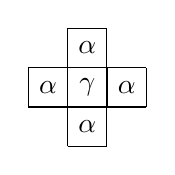
\begin{tikzpicture}
					\draw[step = 0.5] (0,0) grid (0.5,1.5);
					\draw[step = 0.5] (-0.5,1) grid (1,0.5);
					\draw (0.25,1.25) node {$\alpha$};
					\draw (0.25,0.75) node {$\gamma$};
					\draw (0.25,0.25) node {$\alpha$};
					\draw (-0.25,0.75) node {$\alpha$};
					\draw (0.75,0.75) node {$\alpha$};
				\end{tikzpicture}} \text{ mit } \gamma = 1 - 4 \alpha
			\end{equation*}
		
			\begin{equation}
				u_{ij} = (1 - 4 \alpha)f_{ij} + \alpha(f_{i-1,j} + f_{i,j-1} + f_{i,j+1} + f_{i+1,j})
			\end{equation}
		
			\begin{equation*}
					\text{Erinnerung: } \raisebox{-1.2cm}{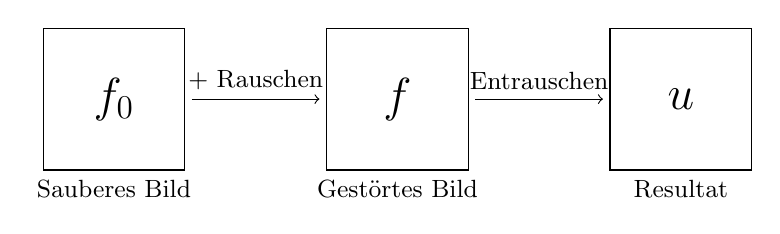
\begin{tikzpicture}[scale=0.9]
						\draw (0,0) rectangle (2,2);
						\draw (1,0) node[below] {\small Sauberes Bild};
						\draw (1,1) node[] {\LARGE $f_0$};
						\draw[->] (2.1,1) -- node[above] {\small $+$ Rauschen} (3.9,1);
						\draw (4,0) rectangle (6,2);
						\draw (5,0) node[below] {\small Gestörtes Bild};
						\draw (5,1) node[] {\LARGE $f$};
						\draw[->] (6.1,1) -- node[above] {\small Entrauschen} (7.9,1);
						\draw (8,0) rectangle (10,2);				
						\draw (9,0) node[below] {\small Resultat};
						\draw (9,1) node[] {\LARGE $u$};
					\end{tikzpicture}}
			\end{equation*}
		
			Annahme: $f_{ij} = f_{ij} +r_{ij}$ mit $r_{ij} \sim N(0,\sigma^2)$ iid.
		
			z.z.: $Var(u_{ij}) \leq Var(f_{ij})$\\
			
			\begin{equation*}
				Var(f_{ij}) = E(\underbrace{f_{ij} - \overbrace{E f_{ij}}^{f^0_{ij}}}%
					_{r_{ij}})^2 = \sigma^2
			\end{equation*}
		
			\todoLayout
			\begin{align*}
				Var(u_{ij}) &= E(u_{ij} - E u_{ij})^2 = E((1 - 4 \alpha) (\underbrace{f_{ij} - f^0_{ij}}_{r_{ij}}) + \alpha(\underbrace{(f_{i-1,j} - f^0_{i-1,j})}_{r_{i-1,j}} + ... + \underbrace{(f_{i+1,j} - f^0_{i+1,j})}_{r_{i+1,j}}))^2\\
				&= E((1 - 4 \alpha)^2 r_{ij}^2 + \alpha^2(r_{i-1,j}^2 + r_{i,j-1}^2 +r_{i,j+1}^2 + r_{i+1,j}^2) + 2 (1 - 4 \alpha) \alpha r_{ij} r_{i-1,j}...)\\
				&= (1 - 4 \alpha)^2 \underbrace{E r_{i,j}^2}_{\sigma^2} + \alpha^2(E r_{i-1,j}^2 + ... + E r_{i+1,j}^2) + 2 (1 - 4 \alpha) \alpha \underbrace{E(r_{ij}r_{i-1,j})}_{\underbrace{E r_{ij} E r_{i-1,j}}_{0}} + \underbrace{...}_{0})\\
				&=(1 - 4 \alpha)^2 \sigma^2 + \alpha^2 4 \sigma^2 = (1 - 8 \alpha + 16 \alpha ^2 + 4 \alpha^2) \sigma^2
			\end{align*}
		
			Da $0 \leq \alpha$ und $ 0 \leq 1 - 4 \alpha \Rightarrow 0 \leq \alpha \leq \frac{1}{4}$:
		
			\begin{equation*}
				(1 - 8 \alpha + 16 \alpha ^2 + 4 \alpha^2) \sigma^2 = \underbrace{1 + \underbrace{20 \alpha}_{\geq 0} (\underbrace{\alpha - \frac{2}{5}}_{< 0})}_{\leq 1}
			\end{equation*}
		
			$\Rightarrow Var(u_{ij}) \leq Var(f_{ij})$ für $\alpha \in [0,\frac{1}{4}]$\\
			
			Dabei gilt: $Var(u_{ij}) \overset{\alpha}{\to} d \text{min} \iff 1 - 8 \alpha + 20 \alpha^2 \overset{\alpha}{\to} \text{min} \iff -8 + 40 \alpha = 0 \iff \alpha = \frac{1}{5}$
		
			\begin{equation*}
				\Rightarrow \text{bester Filter} : \ \raisebox{-0.9cm}{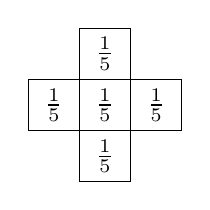
\begin{tikzpicture}[scale = 1.3]
						\draw[step = 0.5] (0,0) grid (0.5,1.5);
						\draw[step = 0.5] (-0.5,1) grid (1,0.5);
						\draw (0.25,1.25) node {$\frac{1}{5}$};
						\draw (0.25,0.75) node {$\frac{1}{5}$};
						\draw (0.25,0.25) node {$\frac{1}{5}$};
						\draw (-0.25,0.75) node {$\frac{1}{5}$};
						\draw (0.75,0.75) node {$\frac{1}{5}$};
					\end{tikzpicture}}
				\end{equation*}

\todoKom{Kapitel sollte noch fehlergelesen werden. 
	Es könnte noch einiges aus dem Skript übernommen werden. 
	Es braucht etwas Layout }

\section{Frequenzfilter}
	\emph{Ansatz}: Rauschen $\approx$ hochfrequente Anteile des Bildes/Signals\\
	\hspace{0.5\linewidth} $\df$ gezieltes entfernen

	\begin{minipage}{1\linewidth}
	 	\tikzpictureQTHIRTYSEVENONE
	\end{minipage}

Wichtiges Instrument: Fouriertransformation (FT)

$$ \mathcal{F} : f \mapsto \hat{f} \text{ mit } \hat{f} (z) = 
	\frac{1}{(2\pi^{\frac{d}{2}}}  \int_{\R^d}dx$$

\todoKom{hier fehlt der rest aus einer Vorlesung}

\todoKom{siehe auch p. 41}

\begin{minipage}{1\linewidth}
% f -> \hat{f} -> u ... 
\end{minipage}

\begin{minipage}{\linewidth}
 % \tikzpictureQFOURTYONETHREE 
\end{minipage}

Genauer: 
$$ \mathcal{F} u = \hat{v} = $$
$$ \begin{aligned}
	g(x) &= \frac{1}{2\pi)^{\frac{d}{2}}} (\inv{\mathcal{F}} \chi_{[-r,r]})(x)\\
			 &= \frac{1}{2\pi)^{\frac{d}{2}}}\frac{1}{2\pi)^{\frac{d}{2}}}
			 		\int_{\R^d} \chi_{[-r,r]}(z) e^{i \fop{z,x} dz} \\
			 & \overset{1d}{=} \frac{1}{2\pi} \int_{-\infty}^{\infty} \chi_{[-r,r]} 
			 	 e^{izx}dz \\
			 &= \frac{1}{2\pi} \int_{-r}^{r} e^{izx} dz 
			 	= \frac{1}{2\pi} \; \frac{e^{izx}}{ix} \bigg| ^r _ {z =-r} \\
			&= \frac{1}{2\pi ix } (e^{irx} - e^{-irx}) = \frac{1}{\pi x} \sin(rx)
\end{aligned}$$	

$$ \hat{g} (0) = (\mathcal{F} g)(0) = \frac{1}{2}$$

\todoKom{allerhand noch im Skript und ein Tafelfoto}

\section{Filterbreite und Glättung}

klar: $\frac{1}{25}$%
\begin{minipage}{0.4\linewidth}
%\tikzpictureQFOURYTFIVEONE
\end{minipage}
glättet mehr als $\frac{1}{9}$%
\begin{minipage}{0.4\linewidth}
%\tikzpictureQFOURYTFIVETWO
\end{minipage}

Im Kontinuierlichen: Sei $m \in L^1(\R^d)$ und $s > 0$.
Setze 
	$$ m_s(x) := \frac{1}{s^d} m (\frac{x}{s}), \quad x\in \R^d$$

Bsp (in $d =1 $0):%
\begin{minipage}{0.4\linewidth}
%\tikzpictureQFOURYTFIVETHREE  
\end{minipage}
$\df$
\begin{minipage}{0.4\linewidth}
%\tikzpictureQFOURYTFIVEFOUR
\end{minipage}

Bsp: G \dots Gauß-Kern, Skalierung mit Fehler $s > 0$
$$ \df G_s(x) = \frac{1}{s^d} G( \frac {x} {s} ) = ...$$
\todoKom{siehe S. 45}
Mo 13 Nov 2017 12:57:12 CET

\chapter{6.Kantenerkennung}

\include{Chapters/7.Schaerfen_und_Entfalten}
\chapter{8.Restauration und Inpainting}

\chapter{9.Segementierung}

\newcommand{\quo}[1] {
\glqq #1 \grqq
}

Dieses ist die Zerlegung eines Bildes in verschiedene Objekt.\\
Eine einfach methode hierfür ist das \mim{Historgramm thresholding}:
\begin{center}
  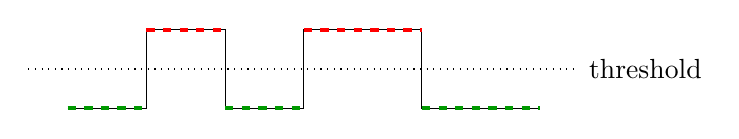
\begin{tikzpicture}
    \draw (1,0) -- (2,0) -- (2,1) -- (3,1) -- (3,0) -- (4,0) -- (4,1) -- (5.5,1) -- (5.5,0) -- (7,0);
    \draw[dotted] (0.5,0.5) -- (7.5,0.5) node[right] {threshold};
    \draw[line width=0.5mm,red,dashed] (2,1) -- (3,1);
    \draw[line width=0.5mm,red,dashed] (4,1) -- (5.5,1);
    \draw[line width=0.5mm,green!60!black,dashed] (1,0) -- (2,0);
    \draw[line width=0.5mm,green!60!black,dashed] (3,0) -- (4,0);
    \draw[line width=0.5mm,green!60!black,dashed] (5.5,0) -- (7,0);
  \end{tikzpicture}
\end{center}
So kann ein Bild in mehrere Objekte zerlegt werden.\\
Hierbei können jedoch diverse Probleme auftreten, die durch preprocessing vermindert werden sollten. Einige der preprocessing methoden sind:
\begin{enumerate}
  \item[-] Entrauschen $\nearrow$ 5.7
  \item[-] Farbraum optimal ausnutzen $\nearrow$ 3.2
  \item[-] \mim{Beleuchtungsausgleich}
\end{enumerate}
Dieser Beleuchtungsausgleich wurde nohc nicht vorher besprochen, das Problem:

\begin{center}
  \begin{tikzpicture}
    \draw (0,0) -- ++(20:1) -- ++(0,1) -- ++(20:1) -- ++(0,-1) -- ++(20:1) -- ++(0,1) -- ++(20:1.5) -- ++(0,-1) -- ++(20:1.5);
    \draw[dotted] (-0.5,1.5) -- (6,1.5) node[right] {threshold??};
  \end{tikzpicture}
\end{center}

Anstatt eines \quo{geraden} Bildes ist das Bild, etwa durch Beleuchtung, \quo{gekippt} und der Ansatz mittels Histogramthresholding würde nicht das gewünschte Ergebniss erzielen.\\

In 2D könnte dies so aus sehen.

\begin{center}
  \begin{tikzpicture}
    \draw[white] (0,0) rectangle node[draw,black] {\includegraphics[scale = 0.2]{images/Bild3plusgrad.png}} (3,3);
    \draw (1.5,3) node[above] {\LARGE $f$};
    \draw (1.5,0) node[below] {gegeben};
    \draw (3.5,1.5) node[] {\LARGE $=$};
    \draw[white] (4,0) rectangle node[draw,black] {\includegraphics[scale = 0.2]{images/Bild3.png}} (7,3);
    \draw (5.5,3) node[above] {\LARGE $u$};
    \draw (5.5,0) node[below] {erwünscht};
    \draw (7.5,1.5) node[] {\LARGE $+$};
    \draw[white] (8,0) rectangle node[draw,black] {\includegraphics[scale = 0.2]{images/Bild3grad.png}} (11,3);
    \draw (9.5,3) node[above] {\LARGE $v$};
    \draw (9.5,0) node[below] {gesucht};
    \draw (11.75,1.5) node[] {\LARGE $\Longleftrightarrow$};
    \draw[white] (12.5,0) rectangle node[draw,black] {\includegraphics[scale = 0.2]{images/Bild3thresh.png}} (15.5,3);
    \draw (14,3) node[above] {};
    \draw (14,0) node[below] {Ergebnis durch thresholding};
  \end{tikzpicture}
\end{center}

Rechts ist das Bild, das durch das Beschreibene Histogramm thresholding dargestellt wurde zu sehen. Methoden um durch preprocessing den gesuchten Gradienten zu entfernen werden im folgenden beschrieben.

\section{Beleuchtungsausgleich}

\begin{enumerate}
  \item[Einfachster Fall:] $v$ konstant. In diesem Fall kann man etwa eine \quo{Leeraufnahme} machen, $v=f$ setzen und dieses $v$ in allen folgenden Aufnahmen subtrahieren.
  \item[Normalfall:] $v$ ändert sich bei Jeder Aufnahme. Hierbei gibt es mehrere Ansätze:
\end{enumerate}

\begin{enumerate}
  \item[a)] \mim{Lineare Regression}: \\
  \begin{minipage}[c]{0.6\linewidth}
          \item[] Wir Unterstellen das der Verlauf \mim{affin-linear} ist, d.h.:
          \[v(x,y) = a x + b y + c\]
          Diese Parameter $a$, $b$, $c$ gilt es nun zu schätzen. 
    \end{minipage}
    \hfill
    \begin{minipage}[c]{0.35\linewidth}
              \begin{center}
        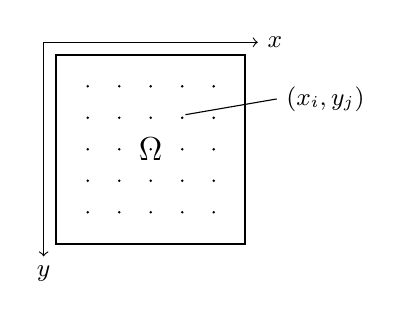
\begin{tikzpicture}[scale=0.8]
          \draw[thick] (0,0) rectangle node[] {\large $\Omega$} (3,3);
          \draw[->] (-0.2,3.2) -- (3.2,3.2) node[right] {\small $x$};
          \draw[->] (-0.2,3.2) -- (-0.2,-0.2) node[below] {\small $y$};
          \foreach \x in {1,...,5}
            \foreach \y in {1,...,5}{
              \draw (\x / 2,\y / 2) node[circle,fill=black,inner sep=0pt] {};
          }
          \draw (2.05,2.05) -- (3.5,2.3) node[right] {\small $(x_i,y_j)$};
        \end{tikzpicture}
      \end{center}
    \end{minipage}
    Dazu soll gelten
    \[\forall (x,y) \in \Omega : ax+by+c \approx f(x,y)\]
    um dieses zu erfüllen wird eine Stichprobe von endlich vielen Punkten $(x_i,y_i)$ aus $\Omega$ gewählt und durch diese ein Gleichungs System gebildet.
    
    \begin{gather*} 
    ax_1+by_1+c \approx f(x_1,y_1)\\
    \vdots \\
    ax_n+by_n+c \approx f(x_n,y_n)
    \end{gather*}
    In Matrix form ergibt sich:
    
    \[\underbrace{\mat{x_1 & y_1 & 1 \\ \vdots & \vdots & \vdots \\ \vdots & \vdots & \vdots \\ \vdots & \vdots & \vdots \\ x_n & y_n & 1}}_{A} \underbrace{\mat{a \\ b \\ c}}_{w} \approx \underbrace{\mat{f(x_1,y_1 \\ \vdots \\ \vdots \\ \vdots \\ f(x_n,y_n)}}_{z}\]
    Die optimale Lösung dieses Problems kann über die \mim{Normalengleichung} berechnet werden.
    
    \[A^T A w = A^T z\]
    
    Dauraus erhält man $w$, somit auch $a$, $b$, $c$ und schlussendlich $v \Rightarrow u = f-v$.\\
    Anschließend wird noch ein Histogram stretching durchgeführt um das finale Bild zu erhalten.
    
    \item[b)] \mim{Polynomiale Regression}:
    Ähnlich zur linearen Regression nun wird hierbei keine affin-lineare Funktion, sondern ein polynom genutzt. Für ein Polynom zwieten gerades kann etwa die Funktion
    \[v(x,y) = ax^2 by^2 cxy+ dx +ey +f\]
    gewählt werden. Wieder entsteht ein Gleichungssytem:
    
    \[\underbrace{\mat{x_1^2 & y_1^2 & x_1y_1 & x_1 & y_1 & 1 \\ \vdots & \vdots & \vdots & \vdots & \vdots & \vdots \\ \vdots & \vdots & \vdots & \vdots & \vdots & \vdots \\ \vdots & \vdots & \vdots & \vdots & \vdots & \vdots \\ x_n^2 & y_n^2 & x_ny_n & x_n & y_n & 1}}_{A} \underbrace{\mat{a \\ b \\ c \\ d \\e \\ f}}_{w} \approx \underbrace{\mat{f(x_1,y_1 \\ \vdots \\ \vdots \\ \vdots \\ f(x_n,y_n)}}_{z}\]

  \item[c)] \mim{Trigonometrisches Polynom}
  Hierbei wird $v$ in den niedrigfrequenten Anteilen von $f$ gesucht.
  
  \begin{center}
    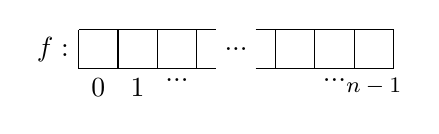
\begin{tikzpicture}
      \draw (0,0.25) node[left] {$f:$};
      \draw[step = 0.5] (0,0) grid (1.75,0.5);
      \draw (2,0.25) node[] {$...$};
      \draw[step = 0.5] (2.25,0) grid (4,0.5);
      \draw (0.25,0) node[below] {$0$};
      \draw (0.75,0) node[below] {$1$};
      \draw (1.25,0) node[below] {$...$};
      \draw (3.25,0) node[below] {$...$};
      \draw (3.75,0) node[below] {\footnotesize $n-1$};
    \end{tikzpicture}
  \end{center}
  
  Es ergibt sich $\hat f$:
  
  \[\hat f_k = \sum_{m=0}^{n-1} f_k \bigl(\underbrace{e^{- i 2 \pi \frac{k}{n}}}_{w_k}\bigr)^m \quad , \ k= 0,1,...,n-1\]
  
  Mittels der FFT (Fast Fourier Transformation) ergibt sich $\hat f$ zu:

  \begin{center}
    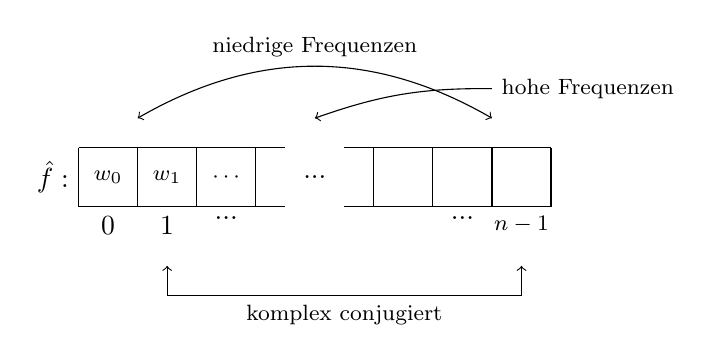
\begin{tikzpicture}[scale=1.5]
      \draw (0,0.25) node[left] {$\hat f:$};
      \draw[step = 0.5] (0,0) grid (1.75,0.5);
      \draw (2,0.25) node[] {$...$};
      \draw[step = 0.5] (2.25,0) grid (4,0.5);
      \draw (0.25,0) node[below] {$0$};
      \draw (0.75,0) node[below] {$1$};
      \draw (0.25,0.25) node[] {\footnotesize $w_0$};
      \draw (0.75,0.25) node[] {\footnotesize$w_1$};
      \draw (1.25,0) node[below] {$...$};
      \draw (3.25,0) node[below] {$...$};
      \draw (1.25,0.25) node[] {\footnotesize$\cdots$};
      \draw (3.75,0) node[below] {\footnotesize $n-1$};
      \draw[<->] (0.75,-0.5) -- (0.75,-0.75) -- node[below] {\footnotesize komplex conjugiert} (3.75,-0.75) -- (3.75,-0.5);
      \draw[<->] (0.5, 0.75) to[bend left] node [above] {\footnotesize niedrige Frequenzen} (3.5,0.75);
      \draw[<-] (2,0.75) to[bend left=10] (3.5,1) node[right] {\footnotesize hohe Frequenzen};
    \end{tikzpicture}
  \end{center}
  Durch entfernen dieser niedrigen Frequenzen ergibt sich $u$.
Ähnliches funktioniert auch in 2D:

    \begin{center}
    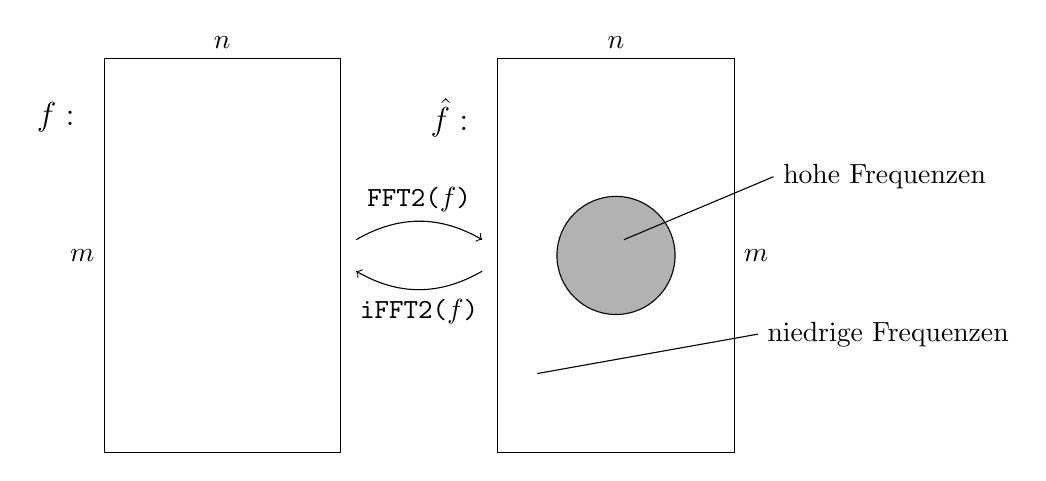
\begin{tikzpicture}[scale=1]
      \draw (0,0) rectangle (3,5);
      \draw (1.5,5) node[above] {$n$};
      \draw (0,2.5) node[left] {$m$};
      \draw (-0.25,4.25) node[left] {\large $f:$};
      \draw[->] (3.2,2.7) to[bend left] node[above] {\tt{FFT2($f$)}} (4.8,2.7);
      \draw[<-] (3.2,2.3) to[bend right] node[below] {\tt{iFFT2($f$)}} (4.8,2.3);
      \draw (5,0) rectangle (8,5);
      \draw (6.5,5) node[above] {$n$};
      \draw (8,2.5) node[right] {$m$};
      \draw (4.75,4.25) node[left] {\large $\hat f:$};
      \draw[fill = black!30] (6.5,2.5) circle (0.75);
      \draw (6.6,2.7) -- (8.5,3.5) node[right] {hohe Frequenzen};
      \draw (5.5,1) -- (8.3,1.5) node[right] {niedrige Frequenzen};
    \end{tikzpicture}
  \end{center}
\end{enumerate}

\chapter{10.Registrierung}

\chapter{11.Mathematischer Nachschlag}
Aus mathematischer Sicht sind einige Fragen offen geblieben, etwa:

\newcommand{\D} {
\mathcal{D}
}

\section{Verallgemeinerte Funktionen und Abbleitungen}
Wie differenziert man unstetige Funktionen?

Sei $\D := C_0^\infty(\R^d)$ die Menge (auch ein Vektorraum) der beliebig oft differenzierbaren Funktionen auf $\R^d$ mit beschränktem Träger. Etwa:

\begin{center}
    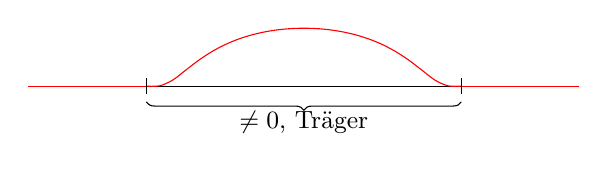
\begin{tikzpicture}
        \draw (-3,0) -- (3,0);
        \draw[scale=2,domain=-0.999:0.999,smooth,variable=\x,red] plot ({\x},{e^(-(1 - abs(\x)^2 )^(-1)});
        \draw[red] (-3.5,0) -- (-0.999*2,0);
        \draw[red] (3.5,0) -- (0.999*2,0);
        \draw (0.999*2,-0.1) -- (0.999*2,0.1);
        \draw (-0.999*2,-0.1) -- (-0.999*2,0.1);
        \draw[decorate,decoration={brace,amplitude=3pt,mirror}] (-2,-0.2) -- node[below] {\small $\neq0$, Träger} (2,-0.2);
    \end{tikzpicture}
\end{center}

Diese Funktion ist:

\[\varphi(x)=g(1- \abs{x}^2)\]

wobei

\[g(t) := \begin{cases}
    e^{\frac{-1}{t}} & ,t>0\\
    0 & ,t\leq 0
\end{cases}\]

Dieses Funktioniert auch im $\R^d$

\def\centerx{2}
\def\centery{-1}

\begin{center}
    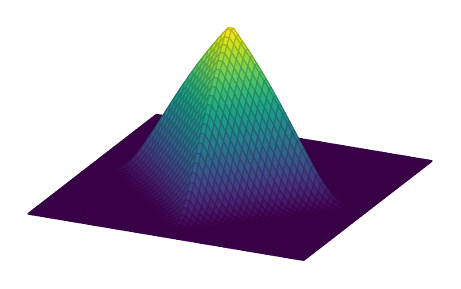
\begin{tikzpicture}[        declare function={
        func(\x) = (\x>0) * e^(-(\x)^(-1)) +
                   (\x<=0) * 0;
      }]

        \pgfplotsset{
            colormap name=viridis,
        }
            \begin{axis}[hide axis,scale=0.75,name=plot1,samples=10]
                \addplot3[surf,domain=-1:1,domain y=-1:1,samples=60]
                    {func(1 - abs(x) - abs(y)))};
                \end{axis}
    \end{tikzpicture}
\end{center}

ist $C_0^\infty(\R^d)$ und hat kompakten Träger.

Sei nun $L^1_{loc}(\R^d)$ die Menge aller Funktionen auf $\R^d$ mit kompaktem Träger für die:

\[\int_K \abs{f(x)} dx < \infty\]

für alle abgeschlossenen und beschränkten Mengen $K \subset \R^d$ gilt.

\begin{center}
    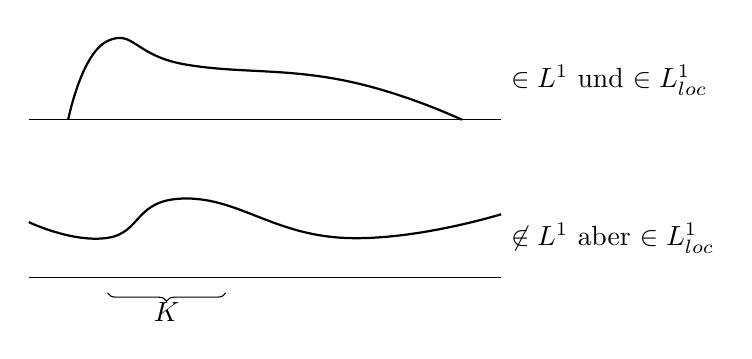
\begin{tikzpicture}
        \draw (-3,0) -- (3,0);
        \draw[thick] plot [smooth, tension = 0.8] coordinates {(-2.5,0) (-2,1)  (-1,0.7) (1,0.5) (2.5,0)};
        \draw (3,0.5) node[right] {$\in L^1$ und $\in L^1_{loc}$};
        \draw (-3,-2) -- (3,-2);
        \draw[thick] plot [smooth, tension = 0.8] coordinates {(-3,-1.3) (-2,-1.5) (-1,-1) (1,-1.5) (3,-1.2) };
        \draw (3,-1.5) node[right] {$\not \in L^1$ aber $\in L^1_{loc}$}; 
        \draw[decorate,decoration={brace,amplitude=3pt,mirror}] (-2,-2.2) -- node[below] {$K$} (-0.5,-2.2);
    \end{tikzpicture}
\end{center}

Die Zweite Funktion ist nicht in $L^1$ da ihr Gesamtintegral nicht endlich ist jedoch ist das Integral über jede endlich Menge endlich, sie hat also keine Pole, somit sie in $L^1_{loc}$.

Für jede Funktion $f \in L^1_{loc}(\R^d)$ bildet 
\begin{equation}\label{eq.11.1}
    \tilde f:\varphi \in \Omega \mapsto \int_{\R^d} f(x) \C \varphi(x) dx \in \R
\end{equation}

ein stetiges lineares Funktional auf $\D$.

Sei nun $\D'$ die Menge aller stetigen linearen Funktionale auf $\D$, also der \mim{Dualraum}. Also ist für jedes $f \in L^1_{loc}$ das Funktional $\tilde f$ aus \eqref{eq.11.1} in $\D'$.

\begin{center}
    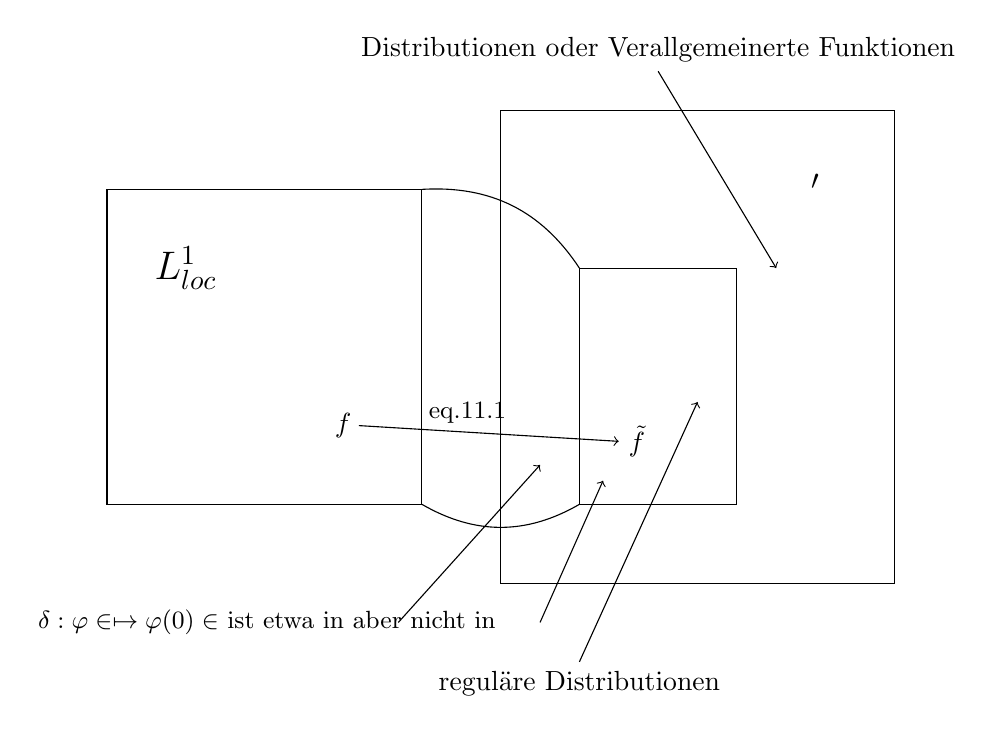
\begin{tikzpicture}
        \draw (0,0) rectangle (4,4);
        \draw (1,3) node[] {\Large $L^1_{loc}$};
        \draw (3,1) node[] {$f$};
        \draw (5,-1) rectangle (10,5);
        \draw (6,0) rectangle (8,3);
        \draw (4,4) to[bend left] (6,3);
        \draw (4,0) to[bend right] (6,0);
        \draw[->] (3.2,1) -- node[above]{\small \eqref{eq.11.1} \ \ \ \ \ } (6.5,0.8) node[right] {$\tilde f$};
        \draw (9,4) node[] {\Large $\D'$};
        \draw[<-] (7.5,1.3) -- (6,-2) node[below]{reguläre Distributionen};
        \draw[<-] (8.5,3) -- (7,5.5) node[above]{\mim{Distributionen} oder Verallgemeinerte Funktionen};
        \draw (-1,-1.5) node[right] {\small $\delta:\varphi \in \D \mapsto \varphi(0) \in \R$ ist etwa in  aber nicht in};
        \draw[<-] (6.3,0.3) -- (5.5,-1.5);
        \draw[<-] (5.5,0.5) -- (3.7,-1.5);
    \end{tikzpicture}
\end{center}

Nun zu den Abbleitungen, sein zunächst $d=1$ und $f \in C^1 \subset L^1_{loc}$, dann gilt für alle $\varphi \in \D$ wobei $[-a,a] \supset supp(\varphi)$:

\[\underbrace{\int_{\R^1} f'(x) \varphi(x) dx}_{f'(\varphi)} = \int_{-a}^a f(x) \phi(x) dx = \underbrace{f(x)\varphi(x)|_{-a}^{a}}_{=0} - \int_{-a}^a f(x) \varphi'(x) dx = -\int_{\R^1} f(x) \varphi'(x) dx = -\tilde f(\varphi')\]

$\Rightarrow$ Für $f \in C^1 \subset L^1_{loc}$ gilt $\tilde f'(\varphi) = - \tilde f(\varphi'), \varphi \in \D$. Wir nehmen dies als Ansatz und setzen:

\begin{equation}\label{eq.11.2}
    F'(\varphi):=-F(\varphi'), \varphi \in \D
\end{equation}

für alle $F\in \D$, genannt Distributionen Abbleitung.

Beispiel:

\begin{center}
    \begin{tikzpicture}
        \draw (-0.4,0) node[left] {$f(x) = \abs{x}$};
        \draw (-0.2,0) -- (4.2,0);
        \draw[thick] (0,2) -- (2,0) -- (4,2);
        \draw (2,-0.1) -- (2,2.3);
    \end{tikzpicture}
\end{center}
Und $F:=\tilde f$ also:

\[F'(\varphi) = -F(\varphi) = - \int_{-a}^a \abs{x} \varphi'(x) dx = - \int_{-a}^0 -x \varphi'(x) dx - \int_0^a x \varphi'(x) dx \]

\[= \int_{-a}^0 x \varphi'(x) dx - \int_0^a x \varphi'(x) dx = \underbrace{x \varphi(x)|_{-a}^0}_{0} - \int_{-a}^0 1 \varphi(x) dx - \underbrace{x \varphi(x)|_0^a}_{0} + \int_0^a 1 \varphi(x) dx\]

\[= \int_{-a}^a sing(x) \varphi(x) dx = \tilde{sign}(\varphi)\]

\begin{center}
    \begin{tikzpicture}
        \draw (-0.4,0) node[left] {$sign(x)=$};
        \draw (-0.2,0) -- (4.2,0);
        \draw (2,-1.3) -- (2,1.3);
        \draw[thick] (2,1) node[left]{\small $1$} -- (4,1);
        \draw[thick] (0,-1) -- (2,-1) node[right]{\small $-1$};
    \end{tikzpicture}
\end{center}

Also insgesamt $F'=\tilde{sign}$

%\clearpage
%\setcounter{page}{1}


%\appendix 

\end{document}
